\documentclass[12pt]{article}
% \usepackage[top=1in,left=1in, right = 1in, footskip=1in]{geometry}
\usepackage[top=1in,footskip=1in]{geometry}

\usepackage{graphicx}
\usepackage{xspace}
%\usepackage{adjustbox}

\usepackage{pdflscape}

\usepackage{grffile}

\newcommand{\comment}{\showcomment}
%% \newcommand{\comment}{\nocomment}

\newcommand{\showcomment}[3]{\textcolor{#1}{\textbf{[#2: }\textsl{#3}\textbf{]}}}
\newcommand{\nocomment}[3]{}

\newcommand{\jd}[1]{\comment{cyan}{JD}{#1}}
\newcommand{\swp}[1]{\comment{magenta}{SWP}{#1}}
\newcommand{\bmb}[1]{\comment{blue}{BMB}{#1}}
\newcommand{\djde}[1]{\comment{red}{DJDE}{#1}}

\newcommand{\eref}[1]{Eq.~(\ref{eq:#1})}
\newcommand{\fref}[1]{Fig.~\ref{fig:#1}}
\newcommand{\Fref}[1]{Fig.~\ref{fig:#1}}
\newcommand{\sref}[1]{Sec.~\ref{#1}}
\newcommand{\frange}[2]{Fig.~\ref{fig:#1}--\ref{fig:#2}}
\newcommand{\tref}[1]{Table~\ref{tab:#1}}
\newcommand{\tlab}[1]{\label{tab:#1}}
\newcommand{\seminar}{SE\mbox{$^m$}I\mbox{$^n$}R}

\usepackage{amsthm}
\usepackage{amsmath}
\usepackage{amssymb}
\usepackage{amsfonts}
\usepackage[utf8]{inputenc} % make sure fancy dashes etc. don't get dropped

\usepackage{lineno}
\linenumbers

\usepackage[pdfencoding=auto, psdextra]{hyperref}

\usepackage{natbib}
\bibliographystyle{chicago}
\date{\today}

\usepackage{xspace}
\newcommand*{\ie}{i.e.\@\xspace}

\usepackage{color}

\newcommand{\Rx}[1]{\ensuremath{{\mathcal R}_{#1}}\xspace} 
\newcommand{\RR}{\ensuremath{{\mathcal R}}\xspace}
\newcommand{\Rres}{\Rx{\mathrm{res}}}
\newcommand{\Rinv}{\Rx{\mathrm{inv}}}
\newcommand{\Rhat}{\ensuremath{{\hat\RR}}}
\newcommand{\Rt}{\ensuremath{{\mathcal R}(t)}\xspace}
\newcommand{\tsub}[2]{#1_{{\textrm{\tiny #2}}}}
\newcommand{\dd}[1]{\ensuremath{\, \mathrm{d}#1}}
\newcommand{\dtau}{\dd{\tau}}
\newcommand{\dx}{\dd{x}}
\newcommand{\dsigma}{\dd{\sigma}}

\newcommand{\rx}[1]{\ensuremath{{r}_{#1}}\xspace} 
\newcommand{\rres}{\rx{\mathrm{res}}}
\newcommand{\rinv}{\rx{\mathrm{inv}}}

\newcommand{\psymp}{\ensuremath{p}} %% primary symptom time
\newcommand{\ssymp}{\ensuremath{s}} %% secondary symptom time
\newcommand{\pinf}{\ensuremath{\alpha_1}} %% primary infection time
\newcommand{\sinf}{\ensuremath{\alpha_2}} %% secondary infection time

\newcommand{\psize}{{\mathcal P}} %% primary cohort size
\newcommand{\ssize}{{\mathcal S}} %% secondary cohort size

\newcommand{\gtime}{\tau_{\rm g}} %% generation interval
\newcommand{\gdist}{g} %% generation-interval distribution
\newcommand{\idist}{\ell} %% incubation-period distribution

\newcommand{\total}{{\mathcal T}} %% total number of serial intervals

\usepackage{lettrine}

\newcommand{\dropcapfont}{\fontfamily{lmss}\bfseries\fontsize{26pt}{28pt}\selectfont}
\newcommand{\dropcap}[1]{\lettrine[lines=2,lraise=0.05,findent=0.1em, nindent=0em]{{\dropcapfont{#1}}}{}}

\begin{document}

\begin{flushleft}{
	\Large
	\textbf\newline{
		Predicting pathogen return to regular cycles 
	}
}
\newline
\\
Sang Woo Park, \dots, Sarah Cobey
\\
\bigskip
\end{flushleft}

\section*{Abstract}

Major priority for epidemiological research in the time of anthropogenic change is understanding how infectious disease dynamics respond to perturbations.
Interventions to slow the spread of COVID-19 significantly disrupted the transmission of other human pathogens, providing unique opportunities to learn about pathogen characteristics from spatiotemporal variation in re-emergence patterns. 
As interventions lifted, a key question of whether and when respiratory pathogens would eventually return to their pre-pandemic dynamics remains to be answered. 
To address this gap, we develop a framework for estimating pathogen resilience based on how fast a pathogen returns to its original cycle.

\pagebreak

Understanding how ecological systems respond to perturbations is a fundamental challenge in predicting the species persistence and extinction.
These responses are often characterized in terms of resilience, which captures how fast a system returns to its stable state following a perturbation.
Both theoretical and empirical efforts to quantify resilience of ecological systems have provided key insights for understanding the dynamics of complex systems and linking these findings to actionable strategies for species conservation.
% However, despite rich literature on ecological resilience, there have been limited applications to measuring the resilience of host-pathogen systems, especially for human pathogens.

Non-pharmaceutical interventions (NPIs) to slow the spread of COVID-19 disrupted the transmission of other human pathogens, providing large-scale natural experiments for understanding how various host-pathogen systems respond to peturbations.
In particular, as interventions lifted, large heterogeneities in outbreak dynamics were observed across different pathogens in different countries (Figure 1), likely reflecting heterogeneities in NPI patterns and pathogen characteristics.
Even though more than four years have already passed since the emergence of COVID-19, many pathogens appear to be far from their regular, seasonal patterns, especially in Hong Kong and South Korea (Figure 1).
These observations pose two fundamental questions for current and future infectious disease dynamics: (1) can we learn something about pathogen characteristics from the patterns of re-emergence? and (2) whether and when other respiratory pathogens would eventually return to their pre-pandemic dynamics?

\begin{figure}[!th]
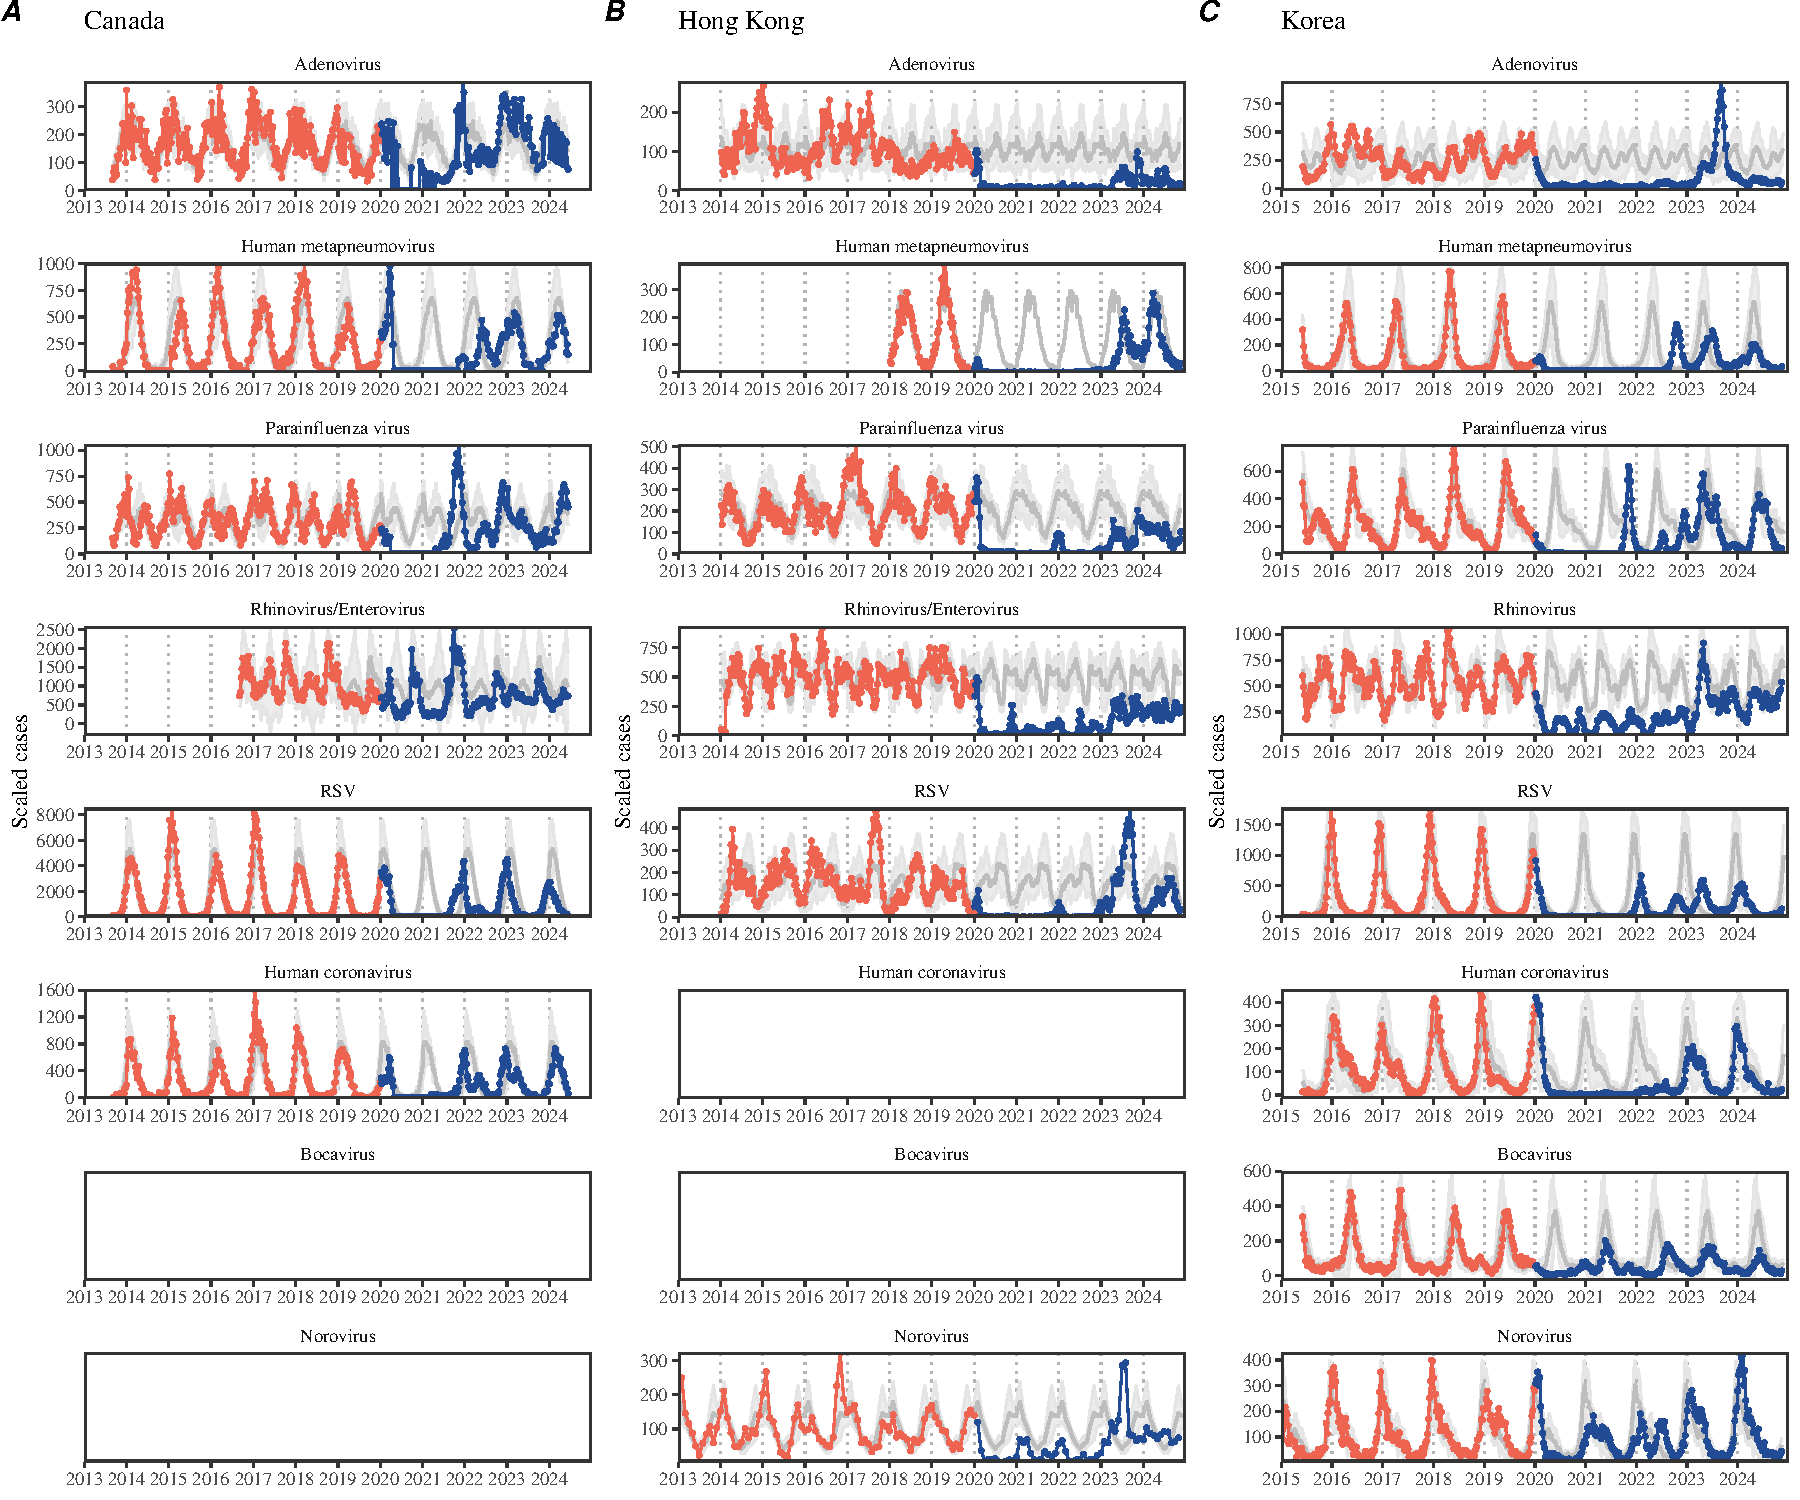
\includegraphics[width=\textwidth]{../figure1/figure1.pdf}
\caption{
\textbf{Observed heterogeneity in responses to COVID-19 pandemic across respiratory pathogens in (A) Canada, (B) Hong Kong, and (C) Korea.}
Red points and lines represent data before 2020.
Blue points and lines represent data since 2020.
Gray lines and shaded regions represent the mean seasonal patterns and corresponding 95\% confidence intervals based on the oberserved outbreak patterns before 2020.
}
\end{figure}

To address this question, we propose a framework for characterizing resilience of a host-pathogen system based on how fast the system recovers from perturbation.
Using simulations, we show that pathogen resilience can provide 

\section*{Conceptual framework for measuring pathogen resilience}

We begin by introducing a conceptual framework for measuring resilience of a host-pathogen system in the cotext of the COVID-19 pandemic and laying out a few important scenarios to set expectations for future dynamics of real-world pathogens.
First, consider an intervention that reduce transmission by 50\% for 6 months starting in 2020, which causes epidemic patterns to deviate from its original stable annual cycle for a short period of time and eventually come back (Figure 2A).
There are many different ways we can characterize this return, but for illustrative purposes, we choose one of the most parsimonious approach: that is, we look at how the susceptible (S) and infected (I) populations change over time and measure the distance on the SI phase plane (Figure 2B).
In this simple case, while the distance from attractor oscillates, its overall rate of return closely matches the \emph{intrinsic} resilience of the system, which represents the expected rate of return and corresponds to the dominant eigenvalue of the underlying model (Figure 2C).

\begin{figure}[!th]
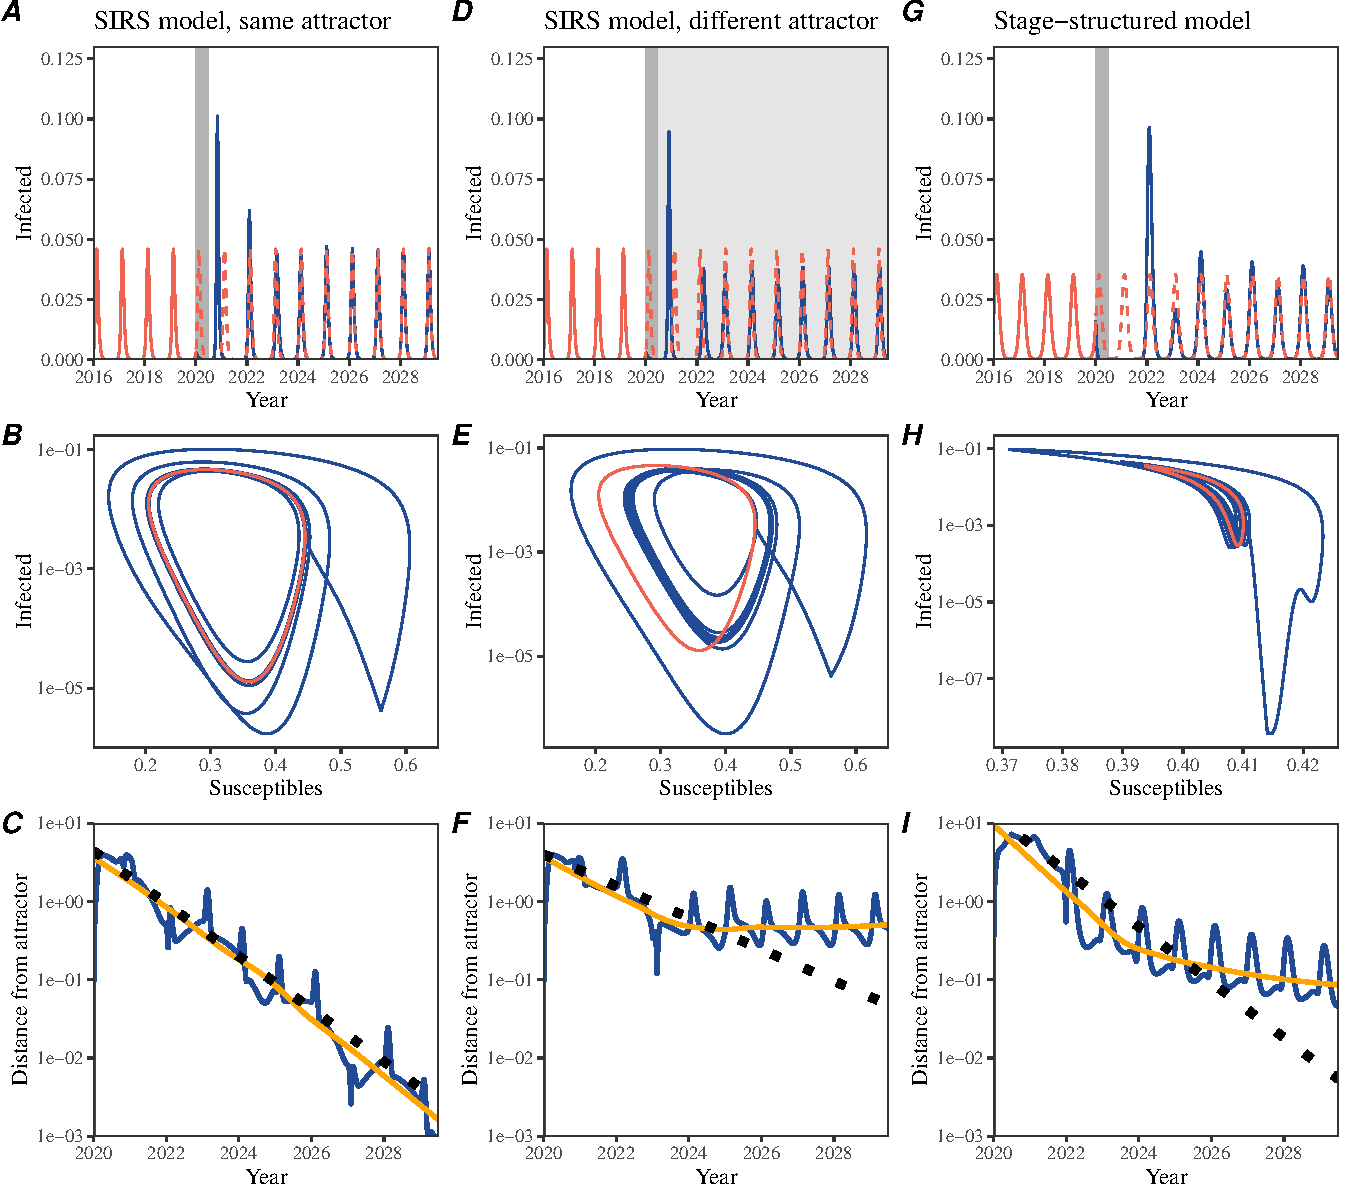
\includegraphics[width=\textwidth]{../figure2/figure2_simple.pdf}
\caption{
\textbf{Conceptual framework for measuring pathogen resilience following NPIs across different scenarios.}
(A, D, G) Simulated epidemic trajectories across various models. 
(B, E, H) Phase plane representation of the corresponding model.
(C, F, I) Changes in logged distance from attractor over time.
}
\end{figure}

Alternatively, NPIs can permanently change our behavior and have persisting impact on the pathogen dynamics; 
as an example, we consider a scenarion in which a 10\% reduction in transmission persists even after the NPIs are lifted (Figure 2D--F).
In such cases, we may not know whether the pathogen will return to its original cycle or a different cycle until many years have passed after the NPIs are lifted, meaning that we cannot measure the distance against the new attractor that the system will be approaching.
Nonetheless, we can still measure the distance against the original, pre-pandemic attractor and still make useful inferences about the system (Figure 2E).
In particular, the distance from the attractor initially decreases exponentially (with oscillations) at a rate that is consistent with the intrinsic resilience of the system (accounting for 10\% reduction in transmission) and eventually plateaus (Figure 2F). 

Transient phenomena can also complicate the picture (Figure 2G--I).
For example, the stage-structured model for RSV initially exhibits a stable annual cycle, but the introduction of NPIs cause the system to exhibit biennial cycles after NPIs are lifted (Figure 2G).
In this case, the distance from the attractor initially decreases exponentially at a rate that is consistent with intrinsic resilience, but the rate of decrease slows down as the epidemic exhibits a biennial cycle (Figure 2I).
In classical ecological theory, this behavior is also referred to as a ghost attractor, which causes long transient dyanmics and slow transitions.

These observations indicate three possibilities.
First, we can directly estimate the empirical resilience of a host-pathogen system by looking at how fast the system approaches an attractor, provided that we have a reasonable way of reconstructing the attractor and calculating the distance from the reconstructed attractor.
The empirical approach to estimating pathogen resilience is particularly convenient because it does not require us to know the true underlying model.
As we show in Supplementary Materials, model misspecification can lead to severe biases in estimation of intrinsic resilience, suggesting that empirical approaches can be more reliable (\swp{TODO}).
Second, resilience estimates allow us to make phenomenological predictions about the dynamics of a host-pathogen system following a perturbation assuming an exponential decrease in the distance from the attractor;
this in turn can be used to estimate when the system will reach the attractor of interest. 
Finally, deviation from an exponential decrease in the distance from attractor can provide information about whether the system has approached an attractor, or a ghost attractor, that is different from the original attractor before perturbation was introduced.

\swp{Multi-strain system to be discussed in the supp after some more investigation.}

\section*{Inferring pathogen resilience from real data}

Based on these obsevations, we now set out to infer pathogen resilience from real data.
To do so, we use Takens' theorem to reconstruct the empirical attractor.
Briefly, Takens' theorem

\begin{figure}[!th]
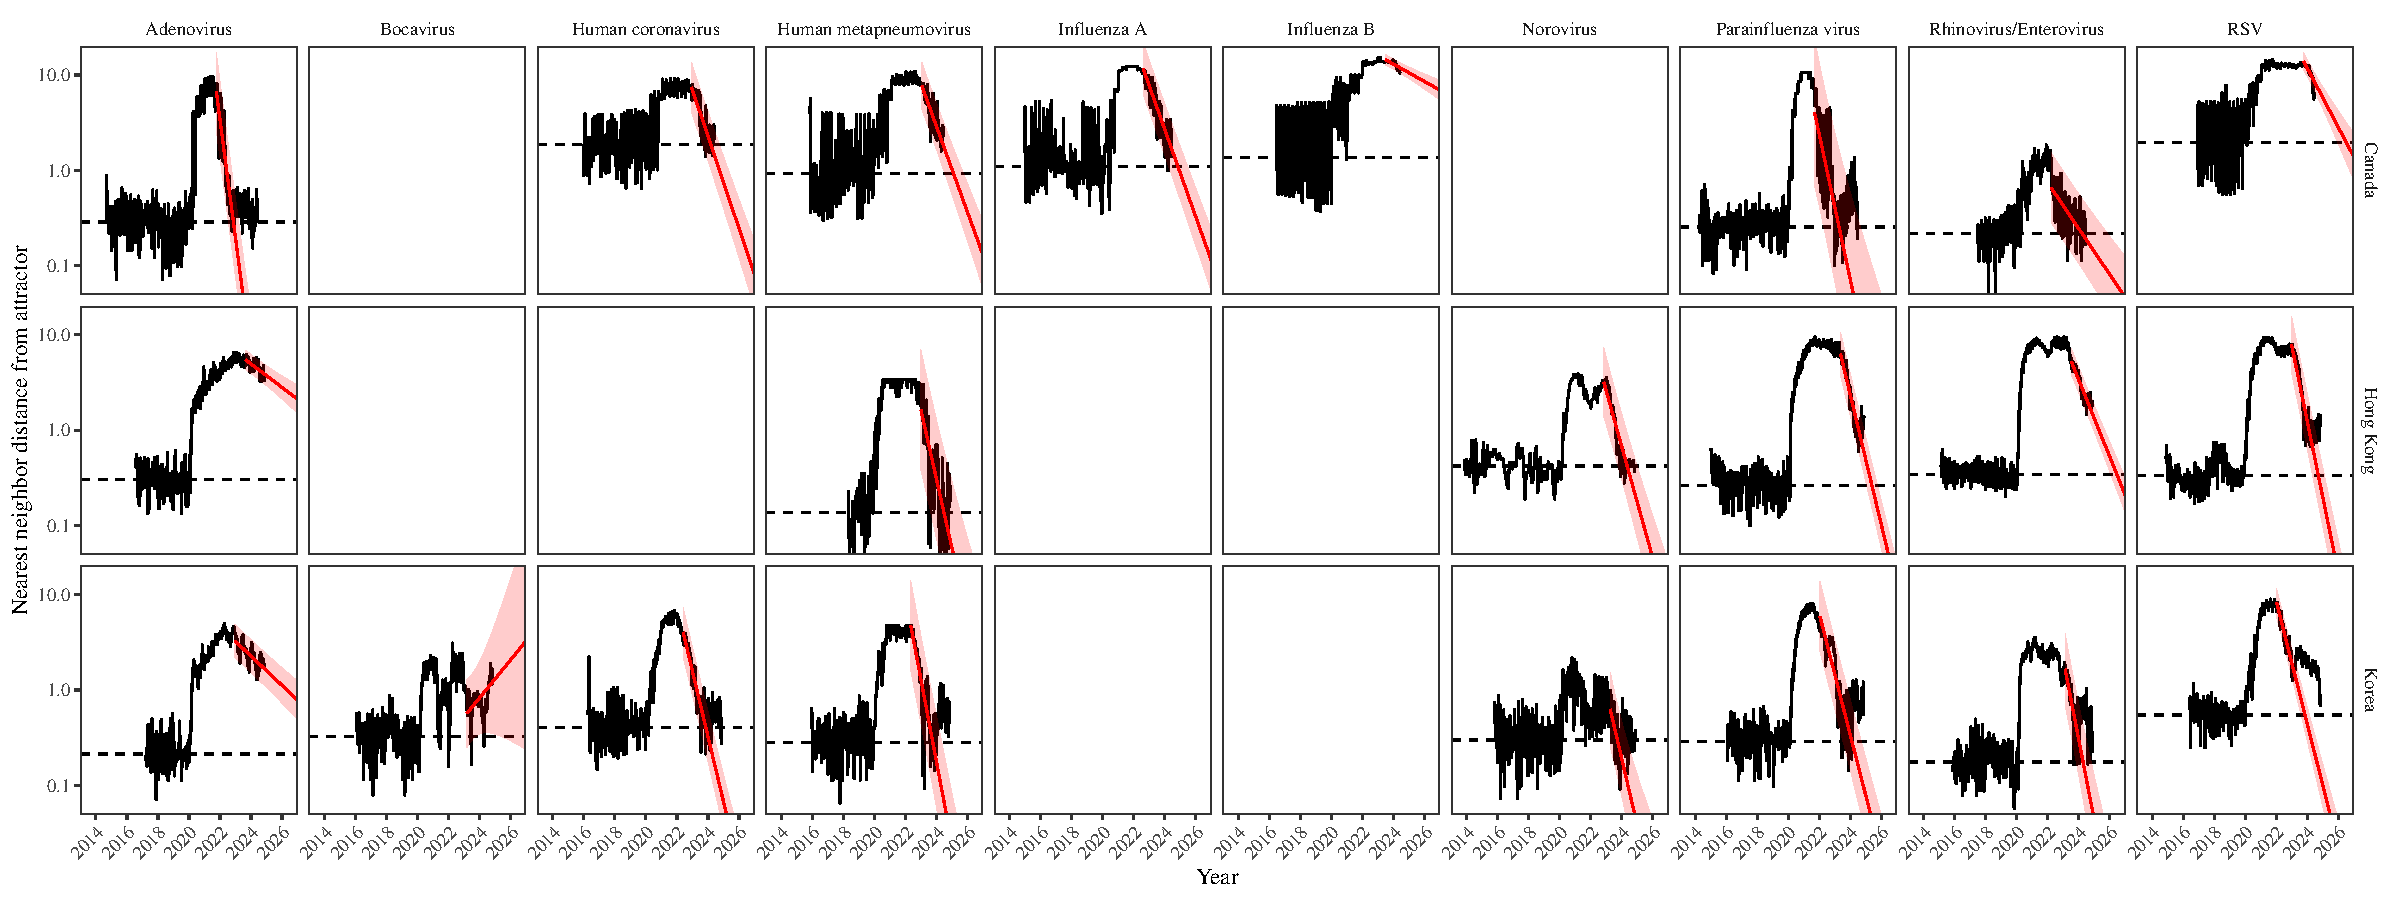
\includegraphics[width=\textwidth]{../figure_takens/figure_takens_acf_fnn_pred.pdf}
\caption{
\textbf{Quantitative framework for estimating pathogen resilience following NPIs.}
}
\end{figure}


\begin{figure}[!th]
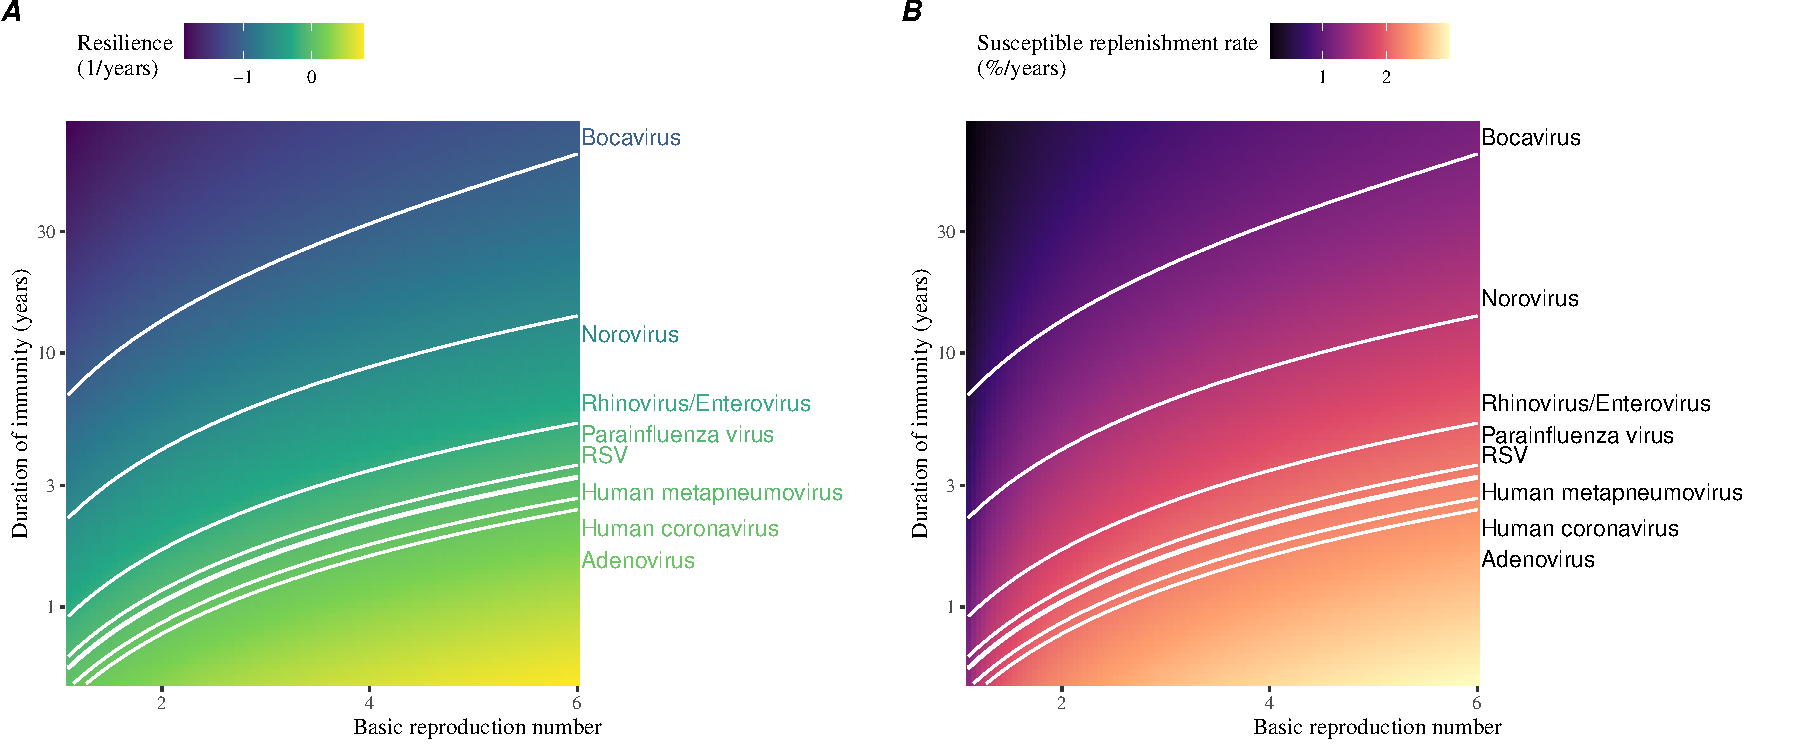
\includegraphics[width=0.5\textwidth]{../figure_summary/figure_summary.pdf}
\caption{
\textbf{Quantitative framework for estimating pathogen resilience following NPIs.}
}
\end{figure}


\end{document}
